\section{Mise DIANA}
\label{sec:mise_diana}
Tato diplomová práce těží z již druhé vesmírné analogové mise, která simulovala
přistání na měsíci a uskutečnila se v rámci projektu Hydronaut v létě roku 2022.
Jednotlivé kompartmenty mise měly následující role: řídící věž byla stanoviště
na Zemi, mateřská loď obíhala na oběžné dráze Měsíce a přistávací modul byl na
povrchu Měsíce. Blíže jsou dílčí kompartmenty popsány v následujících sekcích.

Mise primárně sloužila pro zkoumání vlivu osobnostních charakteristik a vnějších
faktorů na dynamiku týmu při dlouhodobém pobytu v \gls{ICE} prostředí (projekt
TAČR ÉTA č. TL05000228). Mise DIANA byla podpořena Evropskou kosmickou
agenturou, protože by potenciálně mohla umožnit výcvik astronautů právě simulací
extrémního prostředí. 
\subsection{Projekt Hydronaut}
\label{subsec:projekt_hydronaut}
Projekt Hydronaut začal jako podvodní komora, která se postupně proměnila v
laboratoř s celým logistickým a vědeckým zařízením. Nyní slouží pro různorodé
výzkumné účely, včetně zkoumání vlivu izolace a extrémního prostředí na psychiku
člověka a testování technologií za extrémního tlaku.

\subsection{Výběr posádky}
\label{subsec:vyber_posadky}
Výběr posádky pro misi DIANA začal s půlročním předstihem v podobě týmové a
individuální diagnostiky posádky. Tato část byla primárně realizována
psychologickým týmem Filozofické fakulty Univerzity Palackého v Olomouci. Byly
využity neuropsychologické, dotazníkové a škálové metody, přičemž také proběhli
motivační rozhovory na téma pobytu v ICE prostředí. Výsledky testů byly zároveň
použity pro ladění všech psychologických nástrojů a aspektů pro samotnou misi
včetně realizace mise samotné.

Při této příležitosti také proběhly i různorodé technické testy. Všechny
výsledky byly důležité primárně pro přípravu detailního programu celé mise tak,
aby co nejdůvěrohodněji simulovala pobyt v ICE prostředí, včetně minutového
harmonogramu zaměřeného na technické, lékařské, psychologické a sociální
hlediska pobytu. Harmonogram je dále popsán v sekci~\ref{subsubsec:harmonogram_mise}.

\subsection{Posádka pro misi DIANA}
Pro misi DIANA byla vybraná šestice členů posádky. Tři jedinci pro mateřskou loď
a další tři pro podvodní stanici (přistávací modul). Vybraný vzorek se skládal z
mužů ve věkovém rozmezí 20-35 let, kteří předem podstoupili vstupní lékařskou
prohlídku. Výběr proběhl na základě preselekce popsáne v předchozí sekci.
Žádnému jedinci nebyla diagnostikována žádná kardiovaskulární onemocnění, ani
jiné zdravotní problémy, které by mohly být stěžejní pro misi. V rámci posádky
přistávacího modulu se jednalo o trénované potápěče vzhledem k saturačnímu
pobytu po hladinou.

\subsection{Popis lokality a podmínky prostředí}
\label{subsec:diana_lokalita}
Stanice H03 DeepLab je lokalizována v Lomu Jesenný. Obec Jesenný se nachází
severovýchodně od Prahy v okrese Semily, v Libereckém kraji. Jedná se zatopený
vápencový lom o rozloze 130x90~\si\meter~a maximální hloubce 13,5~\si\meter.
Vzhledem k tomu, že mise probíhala pod vodní hladinou, tak nadále nebude uveden
geologický kontext lokality. V průběhu celého experimentu byly příznivé podmínky
počasí a nevyskytli se žádné extrémní události.

\begin{figure}[h]
    \begin{center}
        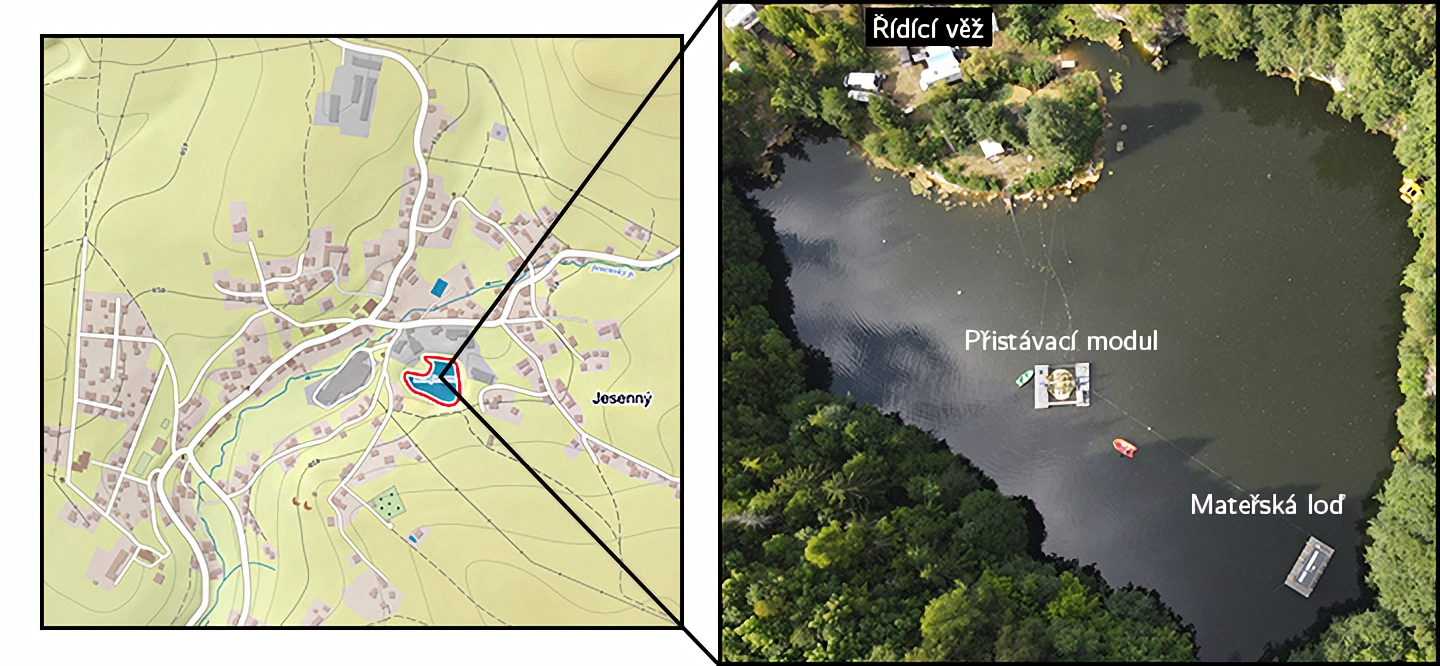
\includegraphics[width=1\linewidth]{figures/map}
        \caption{Detail a lokalita lomu v obci Jesenný (zdroj mapového podkladu: Mapy.cz)}
        \label{fig:map}
    \end{center}
\end{figure}

\subsection{Hlubinná laboratoř H03 DeepLab}
\label{subsubsec:h03_deeplab}
Hydronaut H03 DeepLab je jedinečná výzkumná podvodní laboratoř pro výcvik
posádek v izolovaných, omezených a extrémních podmínkách. Stanice byla zřízena
tak, aby umožnila dlouhodobý pobyt tří členů posádky pod vodní hladinou, přičemž
její konstrukce kombinuje kesonový a ponorkový princip. Díky této unikátní
laboratoří bylo tak umožněno vytvořit podmínky pro dlouhodobý výzkum a sledování
vlivu například tlaku, vlhkosti, stresu, umělého osvětlení a izolovaného
prostředí na člověka nebo použité materiály a vybavení. V rámci mise DIANA plní
roli přistávacího modulu.

\begin{figure}[h]
    \begin{center}
        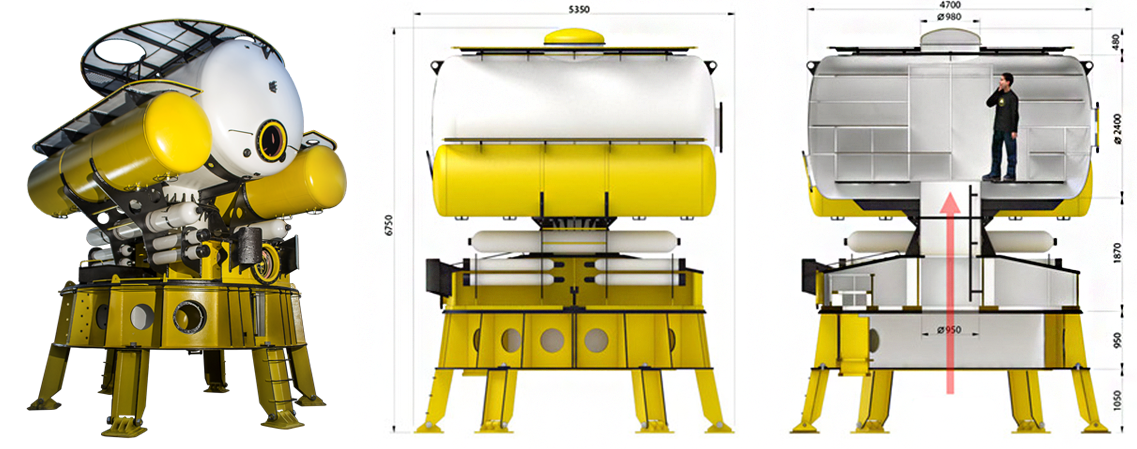
\includegraphics[width=1\linewidth]{figures/habitat}
        \caption{Hlubinná laboratoř H03 DeepLab a její schéma}
        \label{fig:habitat}
    \end{center}
\end{figure}

\subsubsection{Vybavení stanice}
\label{subsubsec:vybaveni_stanice}
Po hardwarové stránce je stanice je vybavena systémy pro monitorování stavu
prostředí uvnitř habitatu a zařízeními pro monitorování fyziologických funkcí
jednotlivých členů posádky. Součástí je také systém pro přenos dat do řídícího
stanoviště.

Pro potřeby například komunikace nebo monitorování fyziologických dat je stanice
vybavena i potřebným softwarem, který je obalen škálovatelným palubním systémem.
Tento systém umožňuje vizualizaci, administraci a hodnocení měřených veličin
(data prostředí, biomedicínská data) společně s obousměrnou komunikaci se všemi
zapojenými účastníky s možností volby různých komunikačních omezení (např. pro
potřeby simulace výpadku komunikace). Vybrané dílčí částí vybavení stanice jsou
detailněji popsány v následujících sekcích.

\subsubsection{Řízení stanice a mise}
\label{subsubsec:rizeni_stanice_mise}
Stanice H03 DeepLab má hlavní komunikační systém zvaný \textit{Common Tongue}.
Ten zajišťuje komunikaci mezi posádkou a podpůrným týmem a umožňuje živé
sledování životních funkcí posádky a vnitřního prostředí. Pomocí tohoto systému
byli subjektům experimentu zadávány úkoly, které jsou sledovány za účelem
vyhodnocení změn chování sledováním vlivu stresu na soustředění a výkonnost
mozku.

\subsubsection{Monitorování atmosféry habitatu}
Jedním z důležitých východisek pobytu v habitatu jsou podmínky prostředí, které
je nezbytné nepřetržitě a spolehlivě monitorovat. Jednou z těchto podmínek je
atmosféra pro jejiž monitorování slouží systém založený na platformě slowRIO
(slow remote IO controller) vyvinutý ve spolupráci s Fakultou strojní (FS ČVUT)
na projektu Hydronaut. Systém monitoruje a poskytuje data prostředí --
mikroklima: absolutní tlak, relativní vlhkost, teplota vzduchu, teplota vody,
čidlo $O_2$, čidlo $CO_2$, čidlo $H_2$, čidlo $CH_4$, intenzita osvětlení, barva
osvětlení a další. Data jsou posílána do palubního počítače.

\subsection{Infrastruktura mise}
\label{subsec:infrastruktura_mise}
Povaha a náročnost stanovených cílů mise se vyžádaly komplexní infrastrukturu
pro podporu celého výzkumného procesu. V této podsekci je uveden stručný přehled
některých součástí infrastruktury včetně harmonogramu mise.

\subsubsection{Harmonogram mise}
\label{subsubsec:harmonogram_mise}
Harmonogram mise byl základním dokumentem, který definoval všechny činnosti v
průběhu mise. Harmonogram byl rozepsaný na úroveň minut pro každého jednotlivého
člena posádky. Ukázku harmonogramu lze vidět na Obr.~\ref{fig:harmonogram}.

\begin{figure}[h]
    \begin{center}
        \begin{framed}
            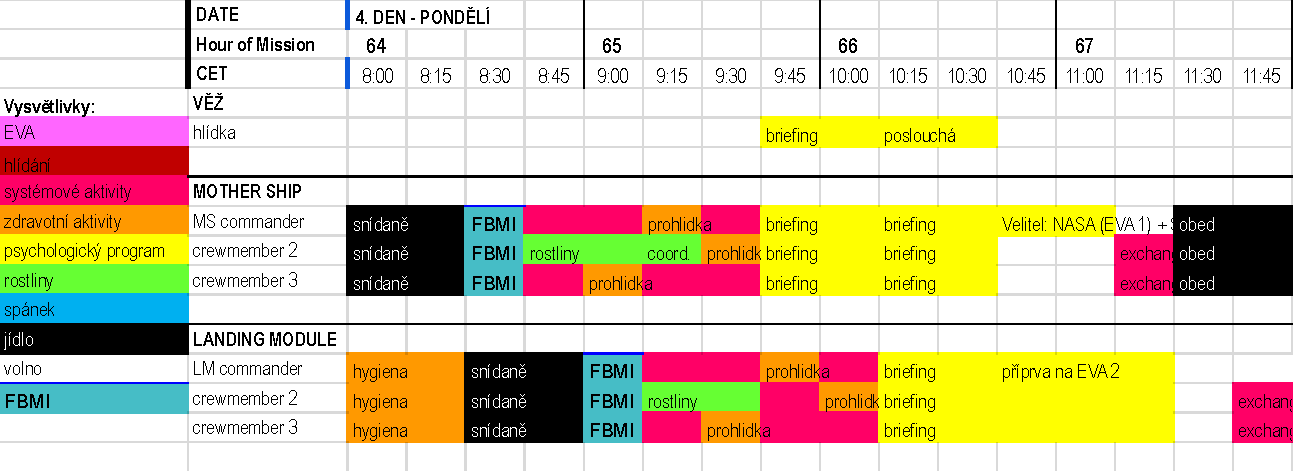
\includegraphics[width=1\linewidth]{figures/harmonogram}
        \end{framed}
        \caption{Ukázka části harmonogramu mise}
        \label{fig:harmonogram}
    \end{center}
\end{figure}

Spolu s harmonogramem byly vytvořeny další dva dokumenty. První z nich byl plán
směn a druhý byl dokument, do kterého se zaznamenávaly všechny významné
události. Plán směn byl vytvořen interně pro každou instituci, jež byla součástí
mise. Každá směna sloužila primárně za účelem monitorování a dokumentace mise.

\subsubsection{Řídicí věž}
\label{subsubsec:ridici_vez}
Řídicí věž hrála v rámci mise DIANA roli stanoviště na Zemi. Komunikovala tedy
se základnou (mateřskou lodí) v souvislosti s prováděním výzkumných a
vzdělávacích programů. Zároveň zde bylo umístěno monitorovací zařízení posádky,
které nepřetržitě sbíralo data a dokumentační a komunikační zařízení.

\begin{figure}[h]
    \begin{center}
        \includegraphics[width=1\linewidth]{figures/monitoring}
        \caption{Monitorování posádky v řídící věži během mise DIANA}
        \label{fig:monitoring}
    \end{center}
\end{figure}

\subsubsection{Povrchová jednotka}
\label{subsubsec:povrchova_jednotka}
Povrchová jednotka byla složena z vedoucího týmu (tři členové stejně jako v
podvodním habitatu), který řídil polohu stanice a systémy podpory života.
Zároveň se povrchová jednotka starala o regulaci specifických parametrů v
závislosti na průběhu mise. Během mise DIANA hrála tato jednotka roli mateřské
lodi, jež sloužila jako stanoviště a kritické zázemí pro velitele posádky. Z
toho místa probíhalo ovládání stanice H03 DeepLab.

\subsection{Neuropsychofyziologická baterie}
\label{subsubsec:neuro_testy}
Neuropsychofyziologická stimulace a diagnostika jedinců byla během mise
realizována prostřednictvím následujících nástrojů:
\begin{enumerate}
    \item \textbf{Kognitivní úlohy v prostředí NEUROP-III} --- posádka opakovaně
          podstoupila náročné diagnostické kognitivní úlohy, zvláště zaměřené na
          sledování exekutivních funkcí primárně v oblasti impulzivního chování,
          riskování, interference nebo inhibice ve smyslu Go-NOGO.
    \item \textbf{Subjektivní hodnocení pomocí NASA TLX} --- jedná se o
          dlouholetý standard pro měření subjektivního vnímání mentální zátěže
          vzhledem ke konkrétním úkolům v pěti dimenzích: mentální náročnost, fyzická
          náročnost, časová náročnost, výkonnost, snaha a frustrace. Posádka byla
          tímto hodnocena během celé mise každý den.
\end{enumerate}

\subsection{Monitorování a měření posádky}
\label{subsec:monitorovani posadky}
Během celého průběhu mise byla posádka neustále monitorována kamerovým systémem
a měřena pomocí validovaných biometrických zařízení, které poskytovaly palubnímu
počítači následující údaje o stavu posádky: tepová frekvence, dechová frekvence,
kožní vodivost. Měření biosignálů je blíže popsáno v další sekci. Zároveň byly
pomocí kamerových záznamů detekovány emoce posádky z výrazů tváře. Na
Obr.~\ref{fig:monitoring} lze vidět snímky z monitorování posádky během mise
DIANA.

\begin{figure}[h]
    \begin{subfigure}[h]{0.48\linewidth}
        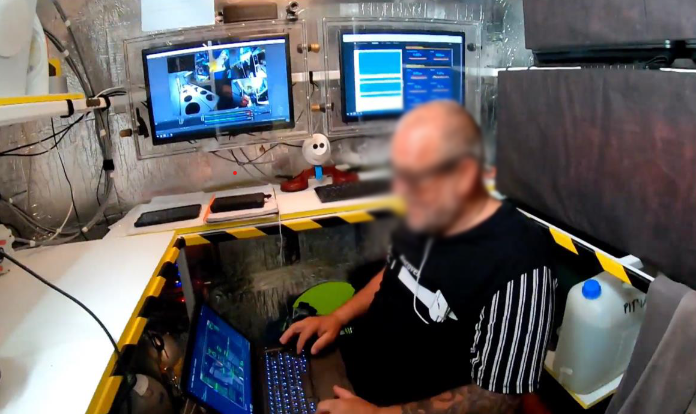
\includegraphics[width=\linewidth]{figures/lander}
        \caption{Snímek z monitorování v přistávacím modulu (interiér modulu)}
    \end{subfigure}
    \hfill
    \begin{subfigure}[h]{0.48\linewidth}
        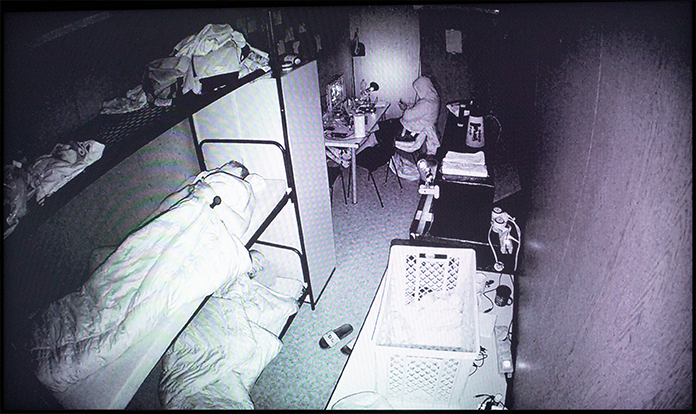
\includegraphics[width=\linewidth]{figures/nightcam}
        \caption{Noční snímek z monitorování posádky mateřské lodi}
    \end{subfigure}
    \caption{Snímky z monitorování posádky během mise DIANA}
\end{figure}

Data z biometrických jednotek byla pomocí bezdrátové síti WLAN (Wi-Fi 2,4 Ghz)
přenášena na datový server a ukládána do InfluxDB. Ostatní kompartmenty mise,
tak mohly živě sledovat fyziologický stav posádky. Díky real-time vizualizaci
bylo také možné dohlížet na správností měření biologických signálů. Předcházelo
se tak situacím jako: nesprávně nalepené či odlepené elektrody, přítomnost
elektromagnetického rušení ovlivňujícího měření nebo výpadky způsobené problémy
s bezdrátovým připojením.

\subsubsection{InfluxDB}
\label{subsec:influx}
InfluxDB\footnote{https://www.influxdata.com} je open-source platforma
poskytující databázi pro časové řady. Zahrnuje rozhraní (API) pro standardní
databázové dotazy. Součástí je i grafické uživatelské rozhraní (GUI) s
modulárními uživatelskými panely pro monitorování dat v reálném čase. Tato
platforma (InfluxDB OSS 2.4) byla využita v rámci mise k uchovávání a
vizualizaci dat.

\subsubsection{Měření biosignálů}
\label{subsubsec:mereni_biosignalu}
V minulé sekci byla zmínka o biometrických datech jako například tepová a
dechová frekvence. Tyto data byla získána pomocí biometrických jednotek, které
však neměří přímo tyto fyziologické indikátory ale biologické signály, konkrétně
srdeční, respirační a elektrodermální aktivitu. Tyto biosignály byly měřeny u
šesti jedinců, konkrétně u posádky mateřské lodi a přistávacího modulu. V
následující sekci je detailněji rozebráno měřící zařízení.

\begin{figure}[h]
    \begin{center}
        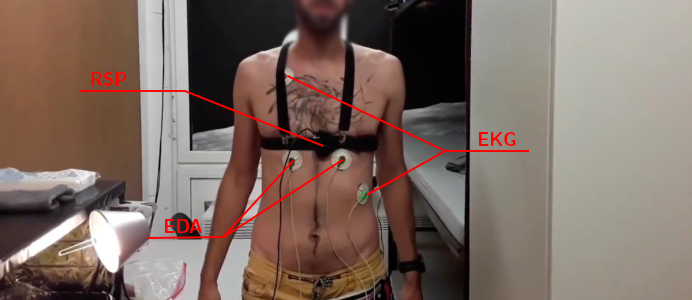
\includegraphics[width=1\linewidth]{figures/sensors}
        \caption{Ukázka měřících čidel na těle člena posádky uvnitř mateřské lodi}
        \label{fig:sensors}
    \end{center}
\end{figure}

\subsubsection{Měřící zařízení}
\label{subsubsec:merici_zarizeni}
Pro měření biosignálu během mise byly použity validované telemedicínské jednotky
\gls{BOREC} (Body recorder), které již dlouhodobě vyvíjíme ve výzkumné skupině
Biomechaniky a asistivních technologií na Fakultě biomedicínského inženýrství
(\gls{FBMI}), ČVUT v Praze. Vzorkovací frekvence zařízení je 250~Hz. Zařízení lze
vidět na Obr.~\ref{fig:borec}.

Respirační aktivita byla měřena pomocí takzvaného dechového pásu, založeného na
tenzometrickém principu. Elektrodermální aktivita byla měřena pomocí dvou
elektrod na hrudi. Toto místo bylo pro potřeby mise vybráno na základě
studie~\cite{Janssen2012}. Elektrická srdeční aktivita byla měřena využitím
jednosvodového systému, přičemž byl svod zaznamenáván v konfiguraci II. Jednotka
včetně snímačů biosignálů také obsahuje tlakové a gyroakcelometrické senzory.

Bezdrátové připojení jednotek je zajištěno díky standardu IEEE 802.11 (Wi-Fi
2,4~GHz). Komunikační protokol mezi zařízením a klientem na straně počítače je
Modbus TCP~\cite{modbus}, který umožňuje přistup k senzorům jednotky a stažení
dat z cyklických redundantních vyrovnávacích pamětí. Každá jednotka má svou
vlastní jedinečnou MAC adresu a očekává adresu IP od serveru DHCP. Klient na PC
má přístup ke všem snímačům místní sítě.

\begin{figure}[h]
    \begin{center}
        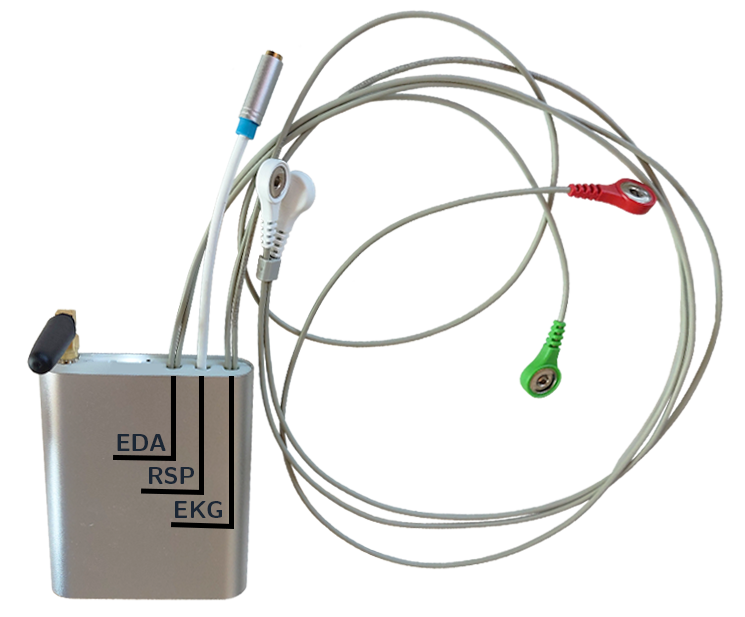
\includegraphics[width=0.65\linewidth]{figures/borec}
        \caption{Telemedicínská jednotka \gls{BOREC} použita během mise}
        \label{fig:borec}
    \end{center}
\end{figure}


\subsection{Studie}
\label{subsec:studie}
%!#TODO: Doplnit referenci na prilohu s informovanym souhlasem
Měření dat probíhalo pod Filozofickou fakultou Univerzity Palackého v Olomouci
(\gls{FF UPOL}). Všichni probandi poskytli informované souhlasy pro část
diagnostickou i pro samotný experiment (viz Příloha~\ref{}). Informované
souhlasy umožňují anonymizované využití dat. Získání dat pod FF UPOL probíhalo
podle etického metakodexu Evropské federace psychologických asociací
(\gls{EFPA}). Informované souhlasy jsou i ke všem nahrávkám obrazových dat a
rozhovorů členů posádky. Bezpečí participantů bylo jištěno v několika
technických rovinách prostřednictvím hlavního řešitele \textit{1st Cloud
Republic a.s.} projektu TL05000228.

\section{Explorační analýza}
\label{sec:exploracni_analyza}

\section{Statistické metody}
\label{sec:statisticke_metody}




% \section{}
% \label{sec:}
% \input{}

% \section{Použité technologie a knihovny}
% \label{sec:technologie_a_knihovny}
% Obory umělé inteligence, jako strojové učení nebo neuronové sítě, často vyžadují
v reálných podmínkách pečlivou přípravu a předzpracování dat nebo sestavení a
trénování modelů. V dnešní době však existuje velké množství nástrojů a
knihoven, které tyto kroky implementují a značně tak zvyšují efektivitu vývoje
patřičných aplikací. Tato kapitola popisuje zásadní nástroje použité pro účely
této práce.

\subsection{Python a R}
\label{subsec:python_r}
Mezi nejpopulárnější open-source programovací jazyky v oblasti strojového učení
a data science, které byly zároveň použity v této práci, patří
Python\footnote{https://www.python.org} a R\footnote{https://www.r-project.org}.
Pro předzpracování dat, strojové učení a neuronové sítě byl použit
Python 3.7 s využitím platformy Google Colab.

Explorační a statistická analýza dat byla realizována prostřednictvím jazyka R
(verze 4.2.1, Funny-Looking Kid) na laptopu \textit{HP Spectre x360} s
procesorem \textit{i7-8705G}, 32~GB DDR4 RAM a grafickou kartou \textit{RX Vega
M GL}. I přestože R není na rozdíl od Pythonu univerzálním vysokoúrovňovým
programovacím jazykem a využívá se především pro statistické modelování, je díky
bohaté komunitě a velkému množství knihoven nedílnou součástí oblasti strojového
učení a data science. 

\subsection{Google Colab a Jupyter Notebook}
\label{subsec:jupyter_colab}
Na základě velkého objemu dat ke zpracování bylo využito platformy Google
Colab\footnote{https://colab.research.google.com}. Jedná se o cloudové
interaktivní výpočetní prostředí, které běží na virtuálním stroji a umožňuje
vzdálené spuštění kódu s využitím prostředků jako \textit{NVIDIA Tesla
V100/P100} s 24~GB VRAM. Jinými slovy jde o hostovanou webovou aplikaci jménem
Jupyter Notebook\footnote{https://jupyter.org}, která umožňuje vytvářet a sdílet
dokumenty (zápisníky). Tyto dokumenty jsou rozděleny do buněk, které lze
spouštět v libovolném pořadí (live kód), což zajišťuje efektivnější
prototypování.

\subsection{Neurokit}
\label{subsec:neurokit}
Knihovna Neurokit2~\cite{Makowski2021neurokit} poskytuje pokročilé metody pro
zpracování a vizualizaci biosignálu. Jednotlivé metody zároveň nabízejí možnost
si vybrat z mnoha implementovaných algoritmů, například pro detekci QRS
komplexu. V této práci byla knihovna použita pro předzpracování respirační,
elektrodermální a srdeční aktivity včetně zpracování HRV.

\subsection{Tidyverse a Easystats}
\label{subsec:tidyverse_easystats}
Knihovny tidyverse~\cite{tidyverse} a easystats~\cite{easystats} rozšiřují jazyk
R o mnoho funkcionalit primárně pro potřeby statistického modelování a
strojového učení. Usnadňují a zrychlují proces tvorby modelů díky dobře
zdokumentovanému ekosystému balíčků. V této práci sloužili knihovny ke
statistické analýze velkého souboru dat. 

\subsection{Scikit-learn, TensorFlow a Keras}
\label{subsec:scitkit_tensor_keras}
Scikit-learn~\cite{sklearn_api} je balíček jazyka Python pro prediktivní analýzu
dat a strojové učení, který byl v této práci použit pro extrakci a normalizaci
příznaků. Dále pro porovnávání, validaci a výběr parametrů a modelů.

% TensorFlow is an open-source framework developed at Google for machine learning
% applications. Its main focus is on defining the architecture and training of
% deep neural networks. It is highly optimized for the execution of low level
% tensor operations on CPU, GPU, or TPU. 

% Keras is a high-level API that acts as an interface for the TensorFlow
% framework. It enables faster prototyping of ANNs by providing abstractions and
% building blocks for developing the models. It also provides the implementation
% of several popular CNN architectures along with their weights, making transfer
% learning more accessible. The simplest way of defining Keras models is by using
% the Sequential model API, which is essentially a linear stack of defined layers.
% The alternative is adopting the Keras functional API, which allows for building
% arbitrary graphs of layers with multiple inputs and outputs or using residual
% skipping connections.

\subsection{InfluxDB}
\label{subsec:influx}
InfluxDB\footnote{https://www.influxdata.com} je open-source platforma
poskytující databázi pro časové řady. Zahrnuje rozhraní (API) pro standardní
databázové dotazy. Součástí je i grafické uživatelské rozhraní (GUI) s
modulárními uživatelskými panely pro monitorování dat v reálném čase. Tato
platforma (InfluxDB OSS 2.4) byla využita v rámci experimentální části práce k
uchovávání a vizualizaci dat.



% \section{Statistické metody}
% \label{sec:_statisticke_metody}
% 



% \begin{figure}[ht]
%     \centering
%     \begin{subfigure}[b]{0.45\textwidth}
%       \mybox{dirs}{%
%       \dirtree{%
%       .1 COVIDx8B.
%       .2 labels.
%       .3 train\_COVIDx8B.txt.
%       .3 test\_COVIDx8B.txt.
%       .2 train.
%       .3 Image\_1.
%       .3 Image\_2.
%       .3 \vdots.
%       .2 test.
%       .3 Image\_1.
%       .3 Image\_2.
%       .3 \vdots.
%       }
%       \tcblower
%       \caption{Original COVIDx8B}
%       \label{subfig:tree1}
%       }
%     \end{subfigure}
%     \begin{subfigure}[b]{0.45\textwidth}
%       \mybox{dirs}{%
%       \dirtree{%
%       .1 COVIDx8B.
%       .2 train.
%       .3 negative.
%       .4 Image\_1.
%       .4 Image\_2.
%       .4 \vdots.
%       .3 positive.
%       .4 Image\_1.
%       .4 Image\_2.
%       .4 \vdots.
%       .2 test.
%       .3 negative.
%       .4 Image\_1.
%       .4 Image\_2.
%       .4 \vdots.
%       .3 positive.
%       .4 Image\_1.
%       .4 Image\_2.
%       .4 \vdots.
%       }
%       \tcblower
%       \caption{Preprocessed COVIDx8B}
%       \label{subfig:tree2}
%       }
%     \end{subfigure}
%     \caption[Comparison of the directory tree of the original COVIDx8B dataset and our preprocessed version]{Comparison of the directory tree of the original COVIDx8B dataset (a) as used by the COVID-Net project, and the preprocessed version (b) which was used in our experiments for image generation during training.}
%     \label{fig:directory_comparison}
%   \end{figure}